\lstinputlisting[firstline=156,lastline=157]{CurryUndMengen.rkt}
\lstinline|(%a %b -> %c)|$\longrightarrow$Applikation auf zwei Argumente (Signaturen \lstinline|%a,%b|) $\longrightarrow$\lstinline|%c|\\
$\left.{\t{Curry}}\Bigg\downarrow\right. \left.\Bigg\uparrow{\t{uncurry}}\right.$\hfill $=\Bigg\updownarrow$ \\
\lstinline|(%a->(%b->%c))|$\rightarrow$App. auf Arg. (Sig. \lstinline|%a|)$\rightarrow$\lstinline|(%b %c)|App. auf Arg. (Sig. \lstinline|%b|)$\rightarrow$\lstinline|%c|\\
\emph{Currying} (Haskell B. Curry, Moses Schönfinkel)\\
Anwendung einer Prozedur auf ihr erstes Argument liefert Prozedur der restlichen Argumente.\\
Jede n-stellige Prozedur lässt sich in eine alternative curried Prozedur transformieren, die in n Schritte jeweils ein Argument konsumiert. Uncurry ist die umgekehrte Transformation.
\begin{lstlisting}
(: curry ((%a %b -> %c) -> (%a -> (%b -> %c))))
(define curry
  (lambda (f)
    (lambda (x)
      (lambda (y)
        (f x y)))))
(: uncurry (%a -> (%b -> %c) -> (%a %b -> %c)))
(define uncurry
  (lambda (f)
    (lambda (x y)
      ((f x) y))))
\end{lstlisting}
Es gilt für jeder Prozedur p:\\
\lstinline|(uncurry (curry p))| = p \hfill \glqq Schönfinkel Isomorphismus \grqq
\rackett{Einfache Curry Beispiele}{Einfache Anwendung von Curry}{CurryUndMengen}{50}{56}
\emph{Erinnerung:} Bestimmung der ersten Ableitung der rellen Funktion durch Bildung des Differentialqoutienten\\
Bildung des Differentialqoutienten:\\
\begin{minipage}[c]{0.6\textwidth}
\begin{tikzpicture}
\begin{axis}[axis x line =center, axis y line =center,xmin=0,ymin=0,xmax=5,ymax=4,xtick={1,4},xticklabels={$x$,$x+h$},ytick={1.3,2.7},yticklabels={$f(x)$,$f(x+h)$}]
\addplot[samples=50,domain={0:5}] gnuplot[id=diffquot]{1.8 * log(x+1)};
\draw[red](axis cs: 0,0)--(axis cs: 2.7,3.5);
\end{axis}
\end{tikzpicture}\end{minipage}
\begin{minipage}[c]{0.4\textwidth}
\[ \frac{f(x+h) - f(x)}{h} \]
Differenzenquotient\\
Steigung(\begin{tikzpicture}
\draw[red](0,0)--(0.2,.2);
\end{tikzpicture})\\
$$\lim\limits_{h \to 0} \frac{f(x+h) - f(x)}{h} = f'(x)$$
\end{minipage}
Operator ' (Ableitung konsumiert Funktionen und produziert Funktion)$\rightarrow$\_' ist higher Order
\rackett{Ableitungen berechnen mit Curry}{Ableitungen mit Curry}{CurryUndMengen}{61}{97}
\emph{Charakteristische Funktion} einer Menge $S \subset M$
\raisebox{-0.5cm}{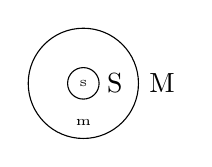
\begin{tikzpicture}
\node () at (0,0) {\tiny s};
\node () at (0.4,0) {S};
\node () at (1,0) {M};
\node () at (0,-0.5) {\tiny m};
\draw circle (0.7);
\draw circle (0.2);
\end{tikzpicture}}\\
Charakteristische Funktion für S: \lstinline[mathescape]|(:$\chi_s$ (M -> Boolean))|\\
$\chi_s(x) = \begin{cases}
\t{\lstinline|#t|} & x \in S\\
\t{\lstinline|#f|} & \t{sonst}
\end{cases}$\\
$\chi_s(m) = \t{\lstinline|#f|}$\qquad $\chi_s(s) = \t{\lstinline|#t|}$\\
Idee Repräsentiere $S \subseteq$ durch Prozedur \lstinline|(M -> boolean)| und Mengenoperation auf Prozeduren (H.O.P)
\rackett{Mengenoperationen Teil 1}{Grundlagen Mengenimplementierung}{CurryUndMengen}{100}{123}
\begin{enumerate}[:-)]
\i Darstellung unendlicher Mengen ($S_42 = \{x \in \mathbb{Z} \mid x > 42 \})$
\i Mengenoperationen $(\cup,\cap,\setminus)$ in \emph{Konstanter Zeit}
\end{enumerate}
Element $x$ in Menge S einfügen:\\
$\chi_{S \cup \{ x \}}(y) = \begin{cases}
\t{\lstinline|#f|} & x =y\\
\chi_s(y) & \t{sonst}
\end{cases}$
\rackett{Mengenoperationen Teil 2}{Erweiterte Mengenoperationen}{CurryUndMengen}{124}{155}